% Compilation Instructions:
% pdflatex paper.tex
% bibtex paper
% pdflatex paper.tex  
% pdflatex paper.tex

\documentclass[conference]{IEEEtran}
\IEEEoverridecommandlockouts
\usepackage{cite}
\usepackage{amsmath,amssymb,amsfonts}
\usepackage{algorithmic}
\usepackage{graphicx}
\usepackage{textcomp}
\usepackage{xcolor}
\usepackage{tabularx}   % for tabularx environment
\usepackage{booktabs}   % for \toprule, \midrule, \bottomrule
\usepackage{multirow}
\usepackage{array}
\usepackage{enumitem}
\usepackage{url}
\usepackage[utf8]{inputenc}
\usepackage{amssymb} % for math symbols
\usepackage{balance}  % put in preamble


\def\BibTeX{{\rm B\kern-.05em{\sc i\kern-.025em b}\kern-.08em
    T\kern-.1667em\lower.7ex\hbox{E}\kern-.125emX}}

% Define consistent model name formatting
\newcommand{\deepseekr}[1]{\texttt{deepseek-r1:#1}}
\newcommand{\qwenthree}[1]{\texttt{qwen3:#1}}
\newcommand{\gptoss}[2]{\texttt{gpt-oss:#1(#2)}}
\newcommand{\DeepSeekR}{DeepSeek-R1}
\newcommand{\QwendThree}{Qwen3}
\newcommand{\GPToss}{GPT-OSS}

\begin{document}

\title{Deploying Reasoning LLMs for Sentiment Analysis: Architecture Trade-offs on Consumer Hardware}

\author{
\IEEEauthorblockN{Donghao HUANG\textsuperscript{1,2}\IEEEauthorrefmark{*}, Nicole TEO\textsuperscript{1}\IEEEauthorrefmark{*}, Aparna CHEKURU\textsuperscript{2}, Erin DEUTSCHMAN\textsuperscript{2}, Zhaoxia WANG\textsuperscript{1}}
\IEEEauthorblockA{
\textsuperscript{1}School of Computing and Information Systems, Singapore Management University, Singapore\\
\textsuperscript{2}Research and Development, Mastercard, Arlington, VA, USA\\
dh.huang.2023@smu.edu.sg, nicolet.2023@engd.smu.edu.sg, aparna.chekuru@mastercard.com, \\ erin.deutschman@mastercard.com, zxwang@smu.edu.sg
}
\thanks{*Equal contribution.}
}

\maketitle

\begin{abstract}
Deploying reasoning large language models (LLMs) for sentiment analysis requires balancing accuracy, explainability, and efficiency under consumer hardware constraints. We present a cross-architecture evaluation of three reasoning model families—DeepSeek-R1, Qwen3, and GPT-OSS—spanning 17 open-weight variants. Using fine-grained Amazon Reviews sentiment classification with few-shot prompting, we benchmark models on an RTX 4090 Laptop GPU (16 GB VRAM) to assess deployment feasibility. We introduce a novel metric---\textit{Reasoning Intensity}---to capture trade-offs between explanation depth and computational cost. Results show that GPT-OSS achieves the highest accuracy (86.2\% F1) but exceeds consumer GPU memory limits, while Qwen3 delivers the most practical balance, with the 8B variant reaching 84.8\% F1 within 13 GB VRAM. Evaluation on a contemporary benchmark reveals consistent 10--15 percentage point F1 degradation across models, though reasoning intensity remains stable over time. Our findings provide evidence-based guidelines for deploying reasoning-enabled, privacy-preserving sentiment analysis on consumer hardware. Code, datasets, and results will be released to support reproducibility.
\end{abstract}

\begin{IEEEkeywords}
sentiment analysis, large language models, explainability, local deployment, reasoning models, consumer hardware, privacy-preserving AI
\end{IEEEkeywords}


\section{Introduction}

Large Language Models (LLMs) have achieved remarkable progress in a wide range of natural language processing (NLP) tasks, including logical fallacy detection~\cite{teo2025large}, logical reasoning~\cite{huang2025logical}, and sentiment analysis~\cite{wang2025review,huang2025explainable}. Recent advancements have introduced reasoning-enabled LLMs, which incorporate intermediate steps or chain-of-thought (CoT) mechanisms to improve interpretability and robustness~\cite{wei2022chain,feng2023towards}. While these models offer better explainability and, in some cases, improved accuracy, they also come with increased computational demands—raising concerns about their deployability on consumer-grade hardware.

In practical applications—particularly in privacy-sensitive domains such as sentiment analysis of user-generated content (e.g., product reviews)—local deployment of models is often preferred, and in some cases, strictly required. The rapid growth of locally deployable large language models (LLMs) has opened new opportunities for privacy-preserving AI, especially in sectors like e-commerce, where sensitive business data cannot be transmitted to external cloud services.

However, deploying state-of-the-art LLMs with reasoning capabilities on consumer-grade GPUs with limited VRAM presents significant challenges. It requires careful trade-offs between model performance (e.g., accuracy), explainability, and computational efficiency.

A key emerging use case is the development of intelligent co-pilots for online sellers—systems designed to analyze customer feedback and support business decision-making while ensuring data privacy through local execution. Yet, transitioning from theoretical capabilities to real-world deployment reveals critical gaps in our understanding of how reasoning-enabled LLMs perform under realistic hardware constraints.

Recent reasoning architectures—including DeepSeek-R1~\cite{guo2025deepseek}, Qwen3~\cite{yang2025qwen3}, and GPT-OSS~\cite{gptoss2025}—introduce new paradigms for explainable sentiment analysis. 
While prior work shows that DeepSeek-R1 delivers strong explainability with competitive accuracy against GPT-4o baselines~\cite{huang2025explainable}, systematic comparisons of reasoning models under consumer hardware remain limited. 
This gap is critical for practitioners who must balance GPU memory, inference latency, and predictive accuracy when deploying privacy-preserving models outside datacenter environments.

Contemporary sentiment analysis faces three converging challenges: (1) the need for transparent and explainable predictions in high-stakes domains, (2) privacy requirements driving local deployment, and (3) hardware constraints that restrict feasible model scales. 
Most existing evaluations target datacenter or cloud settings, leaving practitioners without evidence-based guidelines for consumer hardware deployment.

Building upon established DeepSeek-R1 vs. GPT-4o comparisons~\cite{huang2025explainable}, this work extends evaluation to additional reasoning architectures under consumer hardware constraints through three research questions:
\begin{itemize}[leftmargin=*,nosep]
    \item \textbf{RQ1:} How do contemporary reasoning architectures (DeepSeek-R1, Qwen3, GPT-OSS) compare in sentiment performance, reasoning behavior, and efficiency across scales?  
    \item \textbf{RQ2:} What strategies enable deployment on consumer hardware, and how do VRAM, inference latency, and accuracy trade-offs influence model selection?  
    \item \textbf{RQ3:} How do these models---trained with few-shot learning on the Amazon dataset released 12 years ago~\cite{mcauley2013hidden}---handle temporal drift in contemporary e-commerce reviews?  
\end{itemize}

This work makes four contributions:
\begin{itemize}[leftmargin=*,nosep]
    \item \textbf{Cross-architecture benchmarking:} A systematic evaluation of 17 open-weight reasoning LLMs (DeepSeek-R1, Qwen3, GPT-OSS) for fine-grained sentiment analysis, establishing few-shot baselines under consumer hardware constraints.  
    
    %\item \textbf{Deployment-oriented metrics:} A new measure—\emph{Reasoning Intensity}—to quantify the trade-off between explanation quality, computational cost, and deployment viability. 
    %%%This claim appears to be inaccurate and should be revised. As shown in Table 1, the proposed RI does not seem to reflect the computational cost. It certainly cannot quantify the trade-off between explanation quality, computational cost, and deployment viability. 
    
    %%% for example, 
    %%% model deepseek-r1:8b  RI= 0.873 VRAM=13 GB time=3.71 
    %%% model deepseek-r1:32b RI= 0.873 VRAM=31 GB time=7.05
    %%% model qwen3:4b        RI= 0.825 VRAM=11 GB time=3.93 
    %%% model qwen3:8b        RI= 0.807 VRAM=13 GB time=8.35 
    %%%suggest:
    \item \textbf{Reasoning Intensity (RI) metrics:} A new measure—RI—is proposed to measure a model’s reasoning behavior—for example, how much of its computational cost is devoted to reasoning. RI can be used in conjunction with other metrics (e.g., F1 score [\%], accuracy [\%], time [s], and peak memory usage [GB]) to evaluate trade-offs among explanation quality, computational cost, and deployment viability.
    
    \item \textbf{Empirical deployment analysis:} A detailed study of VRAM–performance–latency trade-offs on consumer hardware, identification of viable models for local deployment, and introduction of a new benchmark (\textit{Testset2}) of contemporary Amazon reviews for temporal robustness evaluation.  
    
    \item \textbf{Open resources.} Code, datasets, and evaluation results are publicly available for reproducibility and further research.\footnote{\url{https://github.com/inflaton/Deploying-Reasoning-LLMs-for-Sentiment-Analysis}}
\end{itemize}

Together, these findings establish a deployment-oriented evaluation framework for reasoning-based sentiment analysis on consumer hardware, providing an empirical foundation for building privacy-preserving e-commerce systems.

\section{Related Work}

LLMs have transformed sentiment analysis, with GPT-based models showing strong zero- and few-shot performance~\cite{brown2020language,zhang2023sentiment} and instruction-tuned variants improving task efficiency~\cite{ghatora2024sentiment}. 
Prompted reasoning approaches, such as chain-of-thought prompting~\cite{lu2024analysis,zhang2025enhancing} and the THOR framework~\cite{fei2023reasoning}, enhance interpretability but rely on careful prompt design and provide limited insight into model internals.
Recent ERC work also explores architecture choices that balance local–global dialogue context with external commonsense, achieving competitive results across standard datasets~\cite{yu2024dialogue}.

\DeepSeekR{} represents a shift toward native reasoning, producing step-by-step traces during inference~\cite{guo2025deepseek}. 
Huang and Wang~\cite{huang2025explainable} show that \DeepSeekR{} surpasses GPT-4o baselines on Amazon Reviews, IMDB, and GoEmotions while embedding explainability directly into the reasoning process. 
New architectures such as \QwendThree{}~\cite{yang2025qwen3} and \GPToss{}~\cite{gptoss2025} introduce distinct trade-offs between accuracy, efficiency, and transparency, yet cross-architecture evaluations under consumer hardware constraints remain scarce.

Few-shot efficiency is increasingly critical for deployment~\cite{huang2024automating,ipa2024bdsentillm}, particularly when API costs or privacy mandates require local execution. 
Consumer GPUs face VRAM bottlenecks, and while quantization enables larger models, its impact under realistic budgets is underexplored. 
Huang and Wang~\cite{huang2025llms} benchmark Qwen2.5 and Llama3 models (0.5B--90B) across diverse hardware with Ollama, finding medium-sized models (7B--32B) best balance performance and efficiency, and quantized models enable edge deployment. 
Complementary software–hardware co-design methods select intermediate representations from frozen LMs under latency and memory constraints, offering a principled path to on-device sentiment and dialogue modeling~\cite{pandelea2023selecting}. 
These results underscore the need for hardware-aware benchmarking to bridge advances in reasoning LLMs with practical, sustainable deployment.

\section{Methodology}

\subsection{Datasets}
\label{sec:datasets}

We evaluate models on the Amazon Reviews sentiment classification task~\cite{mcauley2013hidden}, focusing on fine-grained 5-level sentiment analysis (Strongly Negative, Negative, Neutral, Positive, Strongly Positive). This task requires distinguishing subtle differences in sentiment intensity, making it particularly suitable for assessing reasoning capabilities. 

The fine-grained dataset of 1,838 reviews introduced by~\cite{huang2025explainable} serves as our primary benchmark. It was derived from the original Amazon Reviews corpus through human annotation and split into 70\% training and 30\% testing sets using a fixed random seed (42) for reproducibility. 

To study model robustness under temporal drift, we extend this benchmark with an additional test set. Specifically, we collected public reviews from the same e-commerce platform in mid-2025, anonymized them to remove all personally identifiable information (PII), and randomly sampled 574 reviews. These reviews were manually annotated by trained annotators following the same sentiment classification schema. The resulting dataset, referred to as \textit{Testset2}, provides a contemporary, gold-standard benchmark for evaluating LLMs' generalization capabilities over time.

\subsection{Model Integration}

We evaluate three families of open-weight reasoning LLMs:  
\begin{itemize}[leftmargin=*,nosep]
    \item \textbf{DeepSeek-R1:} 8B, 14B, 32B, and 70B  
    \item \textbf{Qwen3:} 0.6B, 1.7B, 4B, 8B, 14B, 30B, and 32B  
    \item \textbf{GPT-OSS:} 20B and 120B, each available in low, medium, and high reasoning configurations  
\end{itemize}

All models were executed locally via Ollama\footnote{\url{https://ollama.com/}} v0.11.4, using 4-bit quantization (MXFP4 for GPT-OSS models; q4\_K\_M for others), a context length of 8{,}192 tokens, and the framework's default hyperparameters. Model identifiers follow official Ollama naming conventions, e.g., \deepseekr{8b}, \qwenthree{1.7b}, with GPT-OSS models including reasoning effort specifications (low, medium, high), e.g., \gptoss{20b}{low}.

\subsection{Few-shot Prompting}

To ensure methodological consistency, we adopt the few-shot prompting strategy defined in~\cite{huang2025explainable} without modification. Their approach specifies a system prompt template (with placeholders for dataset-specific scale, sentiment labels, and exemplars), a user prompt template, and an exemplar configuration procedure. For few-shot settings, exemplars are sampled from the training set with a fixed random seed (42), stratified to cover all sentiment classes. %This setup enables explainable sentiment classification by requiring the model to output both a predicted label and a brief explanation in JSON format.

\subsection{Hardware Evaluation Framework}

The study employs three hardware platforms:
\begin{itemize}[leftmargin=*,nosep]
\item NVIDIA H100 GPU (96\,GB VRAM)
\item NVIDIA RTX 4090 Laptop GPU (16\,GB VRAM)
\item Apple M3 Max (64\,GB unified memory)
\end{itemize}

All models are first benchmarked on the NVIDIA H100 GPU to establish baseline performance. 
Models that fit within the memory constraints of the RTX 4090 Laptop GPU are subsequently evaluated across all three platforms. 
This cross-platform evaluation measures inference latency and assesses deployment feasibility on consumer hardware.%, with emphasis on privacy-preserving local execution.

The \emph{recommended zone} is defined as models achieving an F1 score of at least 75\% with VRAM usage not exceeding 15\,GB, leaving 1\,GB reserved for system overhead.

\subsection{Evaluation Metrics}

To assess both predictive performance and deployment feasibility, we adopt the following evaluation metrics:

\begin{itemize}[leftmargin=*,nosep]
    \item \textbf{Performance:} Evaluated using weighted F1 score and accuracy on the 5-level sentiment classification task.  
    \item \textbf{Efficiency:} Assessed by inference speed, measured as \emph{Mean Evaluation Time} (in seconds, abbreviated as \emph{Time (s)}), following the definitions in~\cite{huang2025explainable}.  
    \item \textbf{Resource Usage:} Peak VRAM consumption during inference  
    \item \textbf{Reasoning Intensity (RI):} This metric measures the proportion of a model's computational output devoted to reasoning, indicating its reasoning strategy:
\begin{equation}
\text{RI} = \frac{\text{MRT}}{\text{MRT} + \text{MOT}} \label{eq:ri}
\end{equation}

where the components are defined as follows:

\textbf{Mean Reasoning Tokens (MRT):} This metric represents the average number of reasoning tokens a model uses per request, reflecting the extent of its reasoning process:
\begin{equation}
\text{MRT} = \frac{\text{Total Reasoning Tokens}}{\text{Size of Test Dataset}}
 \label{eq:mrt}
 \end{equation}

\textbf{Mean Output Tokens (MOT):} This metric represents the average number of tokens a model generates in its final outputs per request, reflecting its verbosity:
\begin{equation}
\text{MOT} = \frac{\text{Total Output Tokens}}{\text{Size of Test Dataset}} \label{eq:mot}
\end{equation}

RI ranges from 0 to 1, with higher values indicating that a model devotes a greater proportion of its computational output to explicit reasoning processes rather than to producing direct answers.

\end{itemize}

\section{Cross-Architecture Analysis}
\label{sec:cross-arch}

All results in this section are reported on the \emph{standard test set} of the fine-grained Amazon Reviews benchmark~\cite{huang2025explainable}. For \DeepSeekR{} distilled models, we evaluate only the best few-shot configuration as reported in~\cite{huang2025explainable}. 
For all other models, we adopt the same methodology, running 0, 5, 10, 20, 30, 40, and 50 shots to determine the optimal configuration. 

Table~\ref{tab:cross_architecture_results} presents results for all models evaluated on the H100, highlighting distinct reasoning strategies and efficiency trade-offs across architectural paradigms.

\begin{table*}[htbp]
\caption{Cross-Architecture Reasoning Performance (5-Level Sentiment) for Open-weight Models on NVIDIA H100 GPU}
\centering
\begin{tabular}{lcccccccccc}
\toprule
\textbf{Model} & \textbf{F1 (\%)} & \textbf{Acc (\%)} & \textbf{MRT} & \textbf{MOT} & \textbf{RI} & \textbf{VRAM} & \textbf{Time (s)} & \textbf{Shots} \\
\midrule
\multicolumn{9}{c}{\textbf{DeepSeek-R1 Family}} \\
\midrule
deepseek-r1:8b & 71.0 & 68.8 & 338 & 49 & 0.873 & 13 GB & 3.71 & 40 \\
deepseek-r1:14b & 77.4 & 75.5 & 248 & 54 & 0.819 & 18 GB & 4.88 & 30 \\
deepseek-r1:32b & \textbf{81.7} & \textbf{79.9} & 241 & 34 & 0.873 & 31 GB & 7.05 & 50 \\
deepseek-r1:70b & 74.2 & 71.3 & 237 & 40 & 0.855 & 58 GB & 12.08 & 30 \\
\midrule
\multicolumn{9}{c}{\textbf{Qwen3 Family}} \\
\midrule
qwen3:0.6b & 65.2 & 64.8 & 236 & 72 & 0.765 & 6.1 GB & 1.34 & 0 \\
qwen3:1.7b & 75.7 & 76.8 & 217 & 57 & 0.790 & 6.8 GB & 1.56 & 50 \\
qwen3:4b & 84.3 & 83.7 & 284 & 60 & 0.825 & 11 GB & 3.93 & 20 \\
qwen3:8b & \textbf{84.8} & \textbf{84.9} & 249 & 59 & 0.807 & 13 GB & 8.35 & 30 \\
qwen3:14b & 84.6 & 83.7 & 245 & 61 & 0.799 & 19 GB & 10.20 & 30 \\
qwen3:30b & 84.3 & 84.8 & 1234 & 20 & 0.984 & 26 GB & 12.35 & 50 \\
qwen3:32b & 82.3 & 81.3 & 279 & 60 & 0.821 & 40 GB & 15.71 & 30 \\
\midrule
\multicolumn{9}{c}{\textbf{GPT-OSS Family}} \\
\midrule
gpt-oss:20b(low) & 66.9 & 64.2 & 13 & 18 & 0.417 & 23 GB & 0.64 & 40 \\
gpt-oss:20b(medium) & 81.7 & 81.3 & 165 & 28 & 0.851 & 23 GB & 2.30 & 50 \\
gpt-oss:20b(high) & 84.6 & 83.8 & 744 & 30 & 0.961 & 23 GB & 8.60 & 50 \\
gpt-oss:120b(low) & 85.5 & 85.3 & 22 & 40 & 0.361 & 81 GB & 1.58 & 50 \\
gpt-oss:120b(medium) & \textbf{86.2} & \textbf{86.4} & 115 & 42 & 0.728 & 81 GB & 3.15 & 50 \\
gpt-oss:120b(high) & 83.4 & 82.8 & 679 & 43 & 0.940 & 81 GB & 11.84 & 20 \\
\bottomrule
\end{tabular}
\label{tab:cross_architecture_results}

\textbf{Hardware:} NVIDIA H100 GPU (96\,GB VRAM).
\textbf{Evaluation:} Amazon Reviews fine-grained sentiment classification with five labels 
(\textit{Strongly Positive}, \textit{Positive}, \textit{Neutral}, \textit{Negative}, \textit{Strongly Negative}). 
\textbf{Bolded values} indicate the best F1 and accuracy within each model family. 
\textbf{MOT}: Mean Output Tokens (Eq.~\ref{eq:mot}).
\textbf{MRT}: Mean Reasoning Tokens (Eq.~\ref{eq:mrt}).
\textbf{RI}: Reasoning Intensity (Eq.~\ref{eq:ri}).
\textbf{VRAM}: Peak memory usage during inference.
\textbf{Shots}: number of in-context exemplars in the optimal few-shot configuration.
\end{table*}

\subsection{Multi-Family Performance Comparison}

Several critical patterns emerge from our comprehensive evaluation:

\textbf{Architecture Over Scale:} 
Contrary to conventional wisdom that larger parameter counts correlate with higher accuracy, larger models do not always outperform their smaller counterparts. 
Consistent with the findings of~\cite{huang2025explainable}, the \deepseekr{32b} model (80.9\% F1) substantially outperforms the \deepseekr{70b} variant (74.2\% F1), underscoring that architectural efficiency can matter more than parameter count alone. 
A similar trend appears in the \QwendThree{} family, where the \qwenthree{8b} model achieves the highest performance (84.8\% F1), surpassing the \qwenthree{14b}, \qwenthree{30b}, and \qwenthree{32b} variants despite its smaller scale.

\textbf{Reasoning Strategy Diversity:}
The three model families exhibit fundamentally different reasoning strategies:
\begin{itemize}
    \item \textbf{\DeepSeekR} maintains consistent reasoning intensity (avg. 0.858) across model sizes, with moderate token usage (237--338 tokens).
    
    \item \textbf{\QwendThree} demonstrates high baseline performance with efficient reasoning, except for the \qwenthree{30b} variant which uses 1234 reasoning tokens—5× more than other family members—yet achieves comparable performance.
    
    \item \textbf{\GPToss} offers configurable reasoning depth, from minimal (13 tokens) to extensive (744 tokens), enabling application-specific optimization. The \gptoss{120b}{medium} configuration achieves the best overall performance (86.2\% F1) with balanced reasoning (115 tokens).
\end{itemize}

\textbf{Efficiency-Performance Trade-offs:}
Reasoning patterns vary dramatically across architectures:
\begin{itemize}
    \item \gptoss{20b}{low} achieves minimal reasoning through concise processing, suitable for high-throughput applications.
    \item \gptoss{120b}{low} maintains high accuracy (85.2\% F1) with only 22 reasoning tokens, demonstrating that sophisticated models can achieve strong performance without extensive reasoning.
    \item The \qwenthree{30b} model shows inefficient reasoning (RI = 0.984), using excessive tokens without proportional performance gains.
\end{itemize}

\subsection{Reasoning Intensity Analysis}

Figure~\ref{fig:reasoning_intensity} shows the relationship between reasoning intensity (RI) and model performance across architectures. The results reveal three distinct operating regimes.

\begin{figure*}[htbp]
\centering
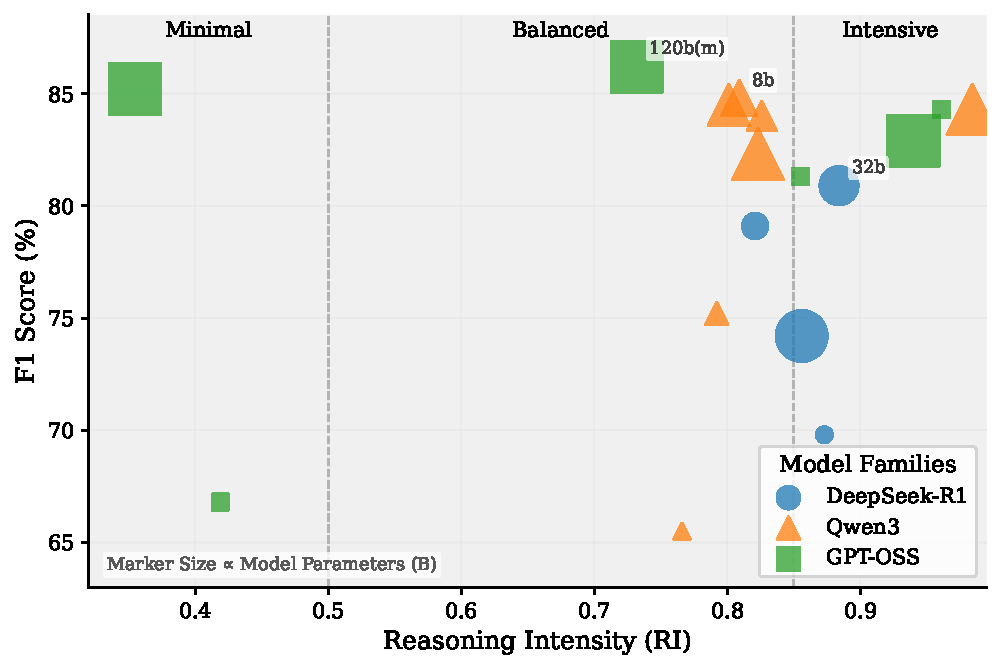
\includegraphics[width=0.9\textwidth]{figures/reasoning_intensity_plot.pdf}
\caption{Relationship between reasoning intensity (RI) and F1 across model families 
($\circ$ DeepSeek-R1, $\triangle$ Qwen3, $\blacksquare$ GPT-OSS). 
Shaded vertical bands mark three operational regimes: \textit{Minimal} (RI $<$ 0.5), 
\textit{Balanced} (0.5--0.85), and \textit{Intensive} (RI $>$ 0.85). 
Marker size scales with parameter count (billions). 
Labels indicate the best-performing configuration within each family. 
GPT-OSS model suffixes denote reasoning effort levels: (l) low, (m) medium, (h) high.}
\label{fig:reasoning_intensity}
\end{figure*}

\textbf{Minimal Reasoning Regime (RI $<$ 0.5):}
Models in this regime prioritize direct output generation over extended reasoning. 
\GPToss{} low-reasoning configurations dominate here, reaching 66.8--85.2\% F1. 
This strategy favors efficiency over interpretability, making it suitable for high-throughput applications.

\textbf{Balanced Reasoning Regime (0.5 $\leq$ RI $\leq$ 0.85):}
Most top-performing models operate in this regime, balancing reasoning depth with efficiency. 
For example, \gptoss{120b}{medium} (RI = 0.732, F1 = 86.2\%) achieves state-of-the-art performance 
while avoiding the overhead of intensive reasoning.

\textbf{Intensive Reasoning Regime (RI $>$ 0.85):}
\DeepSeekR{} models and several \QwendThree{} variants allocate 85--98\% of tokens to reasoning. 
Although this improves interpretability, accuracy gains are modest: for instance, 
\deepseekr{32b} (RI = 0.884) offers only marginal improvement over less intensive counterparts.

\subsection{Few-Shot Learning Efficiency}

Our analysis highlights substantial variation in few-shot learning requirements across model architectures:

\begin{itemize}
    \item \textbf{Zero-Shot Capability:} Only \qwenthree{0.6b} achieves its best performance without examples, though accuracy remains modest (65.5\% F1), reflecting limited in-context learning ability.
    
    \item \textbf{Few-Shot Efficiency:} \qwenthree{4b} reaches 84.0\% F1 with just 20 shots, outperforming larger models that require 30--50 shots to attain comparable results.

    \item \textbf{Shot Saturation:} Most GPT-OSS configurations plateau at around 50 shots, suggesting diminishing returns from additional examples. An exception is \texttt{gpt-oss:120b(high)}, which peaks at 20 shots---indicating that stronger reasoning capacity reduces dependence on large numbers of examples.
    
    \item \textbf{Architecture-Specific Patterns:} \DeepSeekR{} models consistently require 30--50 shots, whereas \QwendThree{} variants show greater variability (0--50 shots), underscoring differences in pre-training strategies and architectural design.
\end{itemize}

\subsection{Explainability Analysis}
Building upon our previous work~\cite{huang2025explainable}, which demonstrated \DeepSeekR's
superior explainability through native reasoning traces, we now broaden the scope to compare
explainability patterns across selected high-performing configurations from all three model families. 
We analyze reasoning strategies using the same review texts and sentiment ground truths as our prior 
study to ensure controlled comparison across model configurations.

\deepseekr{32b} exhibits the most comprehensive reasoning patterns among distilled variants:
\begin{itemize}[leftmargin=*,nosep]
\item \textbf{Systematic Decomposition:} Breaks down reviews into discrete positive and negative elements before synthesis, as demonstrated in neutral sentiment cases where it systematically weighs product failure against customer service quality
\item \textbf{Temporal Reasoning:} Tracks sentiment evolution across review updates and follows logical progression from initial negative experiences to resolution outcomes
\item \textbf{Uncertainty Acknowledgment:} Explicitly recognizes classification ambiguity, such as distinguishing between "Neutral" and "Negative" when reviews contain mixed signals
\item \textbf{Multi-faceted Analysis:} Separates product performance from pricing concerns, enabling nuanced classification in cases where functional satisfaction conflicts with purchase experience
\end{itemize}

\qwenthree{8b} demonstrates efficient yet systematic reasoning approaches:
\begin{itemize}[leftmargin=*,nosep]
\item \textbf{Balanced Analysis:} Consistent evaluation of both positive and negative aspects within concise reasoning traces
\item \textbf{Contextual Grounding:} Strong attention to specific details like star ratings and temporal progression in reviews
\item \textbf{Clear Decision Logic:} Explicit reasoning chains leading to final classifications with transparent justification
\item \textbf{Efficiency Focus:} Maintains reasoning quality while optimizing for faster inference compared to larger variants
\end{itemize}

\GPToss{} models exhibit distinct reasoning behaviors across their configuration settings:
\begin{itemize}[leftmargin=*,nosep]
\item \gptoss{120b}{low}: Minimal reasoning optimized for throughput, with abbreviated decision processes that prioritize speed over explanation depth
\item \gptoss{120b}{medium}: Structured decision-making with moderate detail, systematically weighing factors while maintaining efficiency—representing the optimal balance for this model family
\item \gptoss{20b}{high}: Extensive reasoning traces with detailed analysis and self-referential validation, demonstrating how smaller models can achieve reasoning depth through intensive configuration
\end{itemize}

Comparative analysis across these selected configurations reveals systematic differences in handling 
classification disagreements. \deepseekr{32b} consistently provides the most detailed justification for 
sentiment boundaries, particularly in cases involving mixed reviews where it explicitly weighs competing 
factors. \qwenthree{8b} achieves comparable reasoning quality with greater efficiency, while \gptoss{120b}{medium} 
represents the optimal throughput-accuracy trade-off within its family. When models disagree with ground truth, 
the reasoning traces often reveal defensible alternative interpretations, suggesting that explanation quality 
can aid in identifying systematic annotation inconsistencies and improving model deployment strategies.

Complete reasoning traces and detailed comparative analysis will be made available in our code repository upon paper acceptance.

\section{Consumer Hardware Deployment Analysis}

\subsection{Recommended Models for Consumer Deployment}

Consumer deployment faces significant hardware limitations. The RTX 4090 Laptop GPU, despite being high-end consumer hardware, provides only 16GB VRAM—a fundamental constraint for model selection. Figure~\ref{fig:vram_tradeoffs} visualizes the three-way trade-off between VRAM requirements, performance, and inference speed.

\begin{figure*}[htbp]
\centering
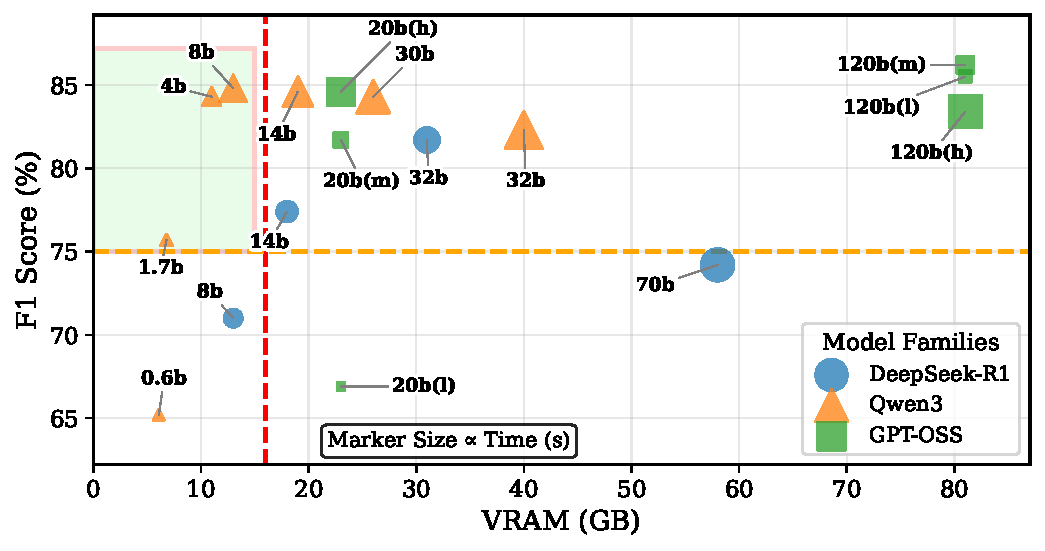
\includegraphics[width=\textwidth]{figures/rtx4090_model_selection.pdf}
\caption{VRAM–performance trade-offs for sentiment analysis models 
($\circ$ DeepSeek-R1, $\triangle$ Qwen3, $\blacksquare$ GPT-OSS). 
VRAM denotes peak memory usage during inference. 
For GPT-OSS, suffixes indicate reasoning effort: (l) low, (m) medium, (h) high. 
Marker size is proportional to mean evaluation time. 
The green shaded area marks the recommended deployment zone (F1 $\geq$ 75\%, VRAM $\leq$ 15\,GB) 
for the RTX 4090 Laptop GPU (16\,GB VRAM). 
The red dashed line represents the 16\,GB memory limit, while the orange dashed line indicates the 75\% F1 threshold. 
Within these constraints, three Qwen3 models are suitable for consumer deployment.}
\label{fig:vram_tradeoffs}
\end{figure*}

Only three models satisfy both performance (F1 $\geq$ 75\%) and hardware (VRAM $\leq$ 15GB) constraints:

\begin{enumerate}[leftmargin=*,nosep]
\item \qwenthree{8b}: Optimal accuracy (84.8\% F1) within hardware limits, 13GB VRAM, 8.35s evaluation time
\item \qwenthree{4b}: Balanced performance (84.3\% F1) with moderate resources (11GB VRAM, 3.93s)  
\item \qwenthree{1.7b}: Resource-constrained deployment (75.7\% F1, 6.8GB VRAM, 1.56s)
\end{enumerate}

\subsection{Cross-Platform Performance Analysis}

To validate our consumer hardware recommendations and assess performance consistency across deployment scenarios, we conducted comprehensive cross-platform evaluation on both the original benchmark and contemporary Amazon reviews. Table~\ref{tab:cross_platform_reasoning_results} presents results across three hardware configurations representing different deployment contexts: H100 for research evaluation, RTX 4090 for consumer deployment, and M3 Max for alternative consumer platforms with unified memory architectures.

\begin{table*}[htbp]
\caption{Cross-Platform Performance Comparison: Original vs. Contemporary Amazon Reviews}
\centering
\begin{tabular}{llcccccccc}
\toprule
\multirow{2}{*}{\textbf{Model}} & \multirow{2}{*}{\textbf{Hardware}} 
& \multicolumn{4}{c}{\textbf{Original Dataset}} 
& \multicolumn{4}{c}{\textbf{Contemporary Dataset (Testset2)}} \\
\cmidrule(lr){3-6} \cmidrule(lr){7-10}
& & \textbf{F1 (\%)} & \textbf{Acc (\%)} & \textbf{RI} & \textbf{Time (s)} 
  & \textbf{F1 (\%)} & \textbf{Acc (\%)} & \textbf{RI} & \textbf{Time (s)} \\
\midrule
\multirow{3}{*}{\texttt{qwen3:1.7b}} 
 & H100     & 75.7 & 76.8 & 0.790 & 1.56 & 57.9 & 62.2 & 0.802 & 1.64 \\
 & RTX 4090  & 72.6 & 73.3 & 0.794 & 1.94 & 58.1 & 63.1 & 0.804 & 2.20 \\
 & M3 Max   & 73.3 & 74.0 & 0.792 & 3.42 & 56.6 & 62.0 & 0.806 & 3.64 \\
\midrule
\multirow{3}{*}{\texttt{qwen3:4b}} 
 & H100     & 84.3 & 83.7 & 0.825 & 3.93 & 67.8 & 69.2 & 0.836 & 2.78 \\
 & RTX 4090  & 81.7 & 81.5 & 0.832 & 3.52 & 65.7 & 67.4 & 0.833 & 3.72 \\
 & M3 Max   & 82.8 & 82.4 & 0.825 & 9.85 & 68.8 & 70.0 & 0.836 & 6.54 \\
\midrule
\multirow{3}{*}{\texttt{qwen3:8b}} 
 & H100     & 84.8 & 84.9 & 0.807 & 8.35 & 72.3 & 73.2 & 0.828 & 3.11 \\
 & RTX 4090  & 82.1 & 82.4 & 0.805 & 4.42 & 73.3 & 74.0 & 0.822 & 5.04 \\
 & M3 Max   & 84.2 & 84.2 & 0.810 & 8.71 & 70.9 & 71.4 & 0.829 & 9.17 \\
\bottomrule
\end{tabular}
\label{tab:cross_platform_reasoning_results}

\vspace{2mm}
\textbf{Evaluation:} Amazon Reviews fine-grained sentiment classification with five labels 
(\textit{Strongly Positive}, \textit{Positive}, \textit{Neutral}, \textit{Negative}, \textit{Strongly Negative}). 
\textbf{RI}: Reasoning Intensity (Eq.~\ref{eq:ri}).
\textbf{Dataset Comparison:} Original dataset refers to the fine-grained Amazon Reviews test set from~\cite{huang2025explainable}. Contemporary dataset (Testset2) contains 574 manually annotated Amazon US reviews collected in mid-2025.\;
\textbf{Hardware:} H100 (96\,GB VRAM), RTX 4090 Laptop GPU (16\,GB VRAM), M3 Max (64\,GB unified memory). All models evaluated using optimal shot configurations determined in Section~\ref{sec:cross-arch}.
\end{table*}


Our cross-platform evaluation reveals several critical insights for consumer hardware deployment:

\textbf{Platform Performance Consistency:} RTX 4090 maintains competitive performance relative to H100 across all model sizes, with minimal degradation (1-3 percentage points F1). This validates the viability of consumer hardware for high-quality sentiment analysis deployment, addressing privacy concerns that necessitate local processing.

\textbf{Temporal Performance Degradation:} All models exhibit a consistent 10--15 percentage point drop in F1 when evaluated on contemporary reviews compared to the original benchmark. Notably, \texttt{qwen3:8b} shows superior resilience to temporal shift, maintaining 72.3--73.3\% F1 on \textit{Testset2} across all platforms—the smallest relative degradation among the evaluated models. Similar degradation has also been observed in other models evaluated on H100. These results are omitted here due to page limits but will be released alongside the code, data, and additional results.

\textbf{Reasoning Patterns:} RI remains stable (±0.02) across temporal domains, suggesting consistent reasoning strategies across temporal domains.

\textbf{Hardware-Specific Performance Characteristics:} M3 Max demonstrates 2-3× inference latency compared to NVIDIA GPU platforms, particularly affecting larger models. However, accuracy remains competitive, making it viable for accuracy-critical applications where inference speed is secondary.

\textbf{Deployment Strategy Recommendations:}
\begin{itemize}[leftmargin=*,nosep]
\item \textbf{Production Systems:} Deploy \texttt{qwen3:8b} on RTX 4090 for optimal accuracy-resource balance (82.1\% F1, 4.42s inference, 13GB VRAM)
\item \textbf{Development/Testing:} Use \texttt{qwen3:4b} for rapid iteration with acceptable accuracy loss (81.7\% F1, 3.52s inference, 11GB VRAM)
\item \textbf{Resource-Constrained Scenarios:} Consider \texttt{qwen3:1.7b} when power consumption or memory constraints are critical (72.6\% F1, 1.94s inference, 6.8GB VRAM)
\end{itemize}

These findings establish evidence-based guidelines for reasoning sentiment analysis deployment under realistic consumer hardware constraints, enabling privacy-preserving local processing without significant performance penalties compared to cloud-based alternatives.

\section{Conclusion}
This work systematically evaluated 17 reasoning LLMs for fine-grained sentiment analysis under consumer hardware constraints. By comparing DeepSeek-R1, Qwen3, and GPT-OSS across multiple scales, we showed how architectural design and reasoning strategies directly affect deployability.  

\textbf{Key takeaways:}
\begin{itemize}
    \item \textbf{GPT-OSS} achieves the highest accuracy (86.2\% F1) but requires $>$23 GB VRAM, exceeding consumer GPU limits.  
    \item \textbf{Qwen3}, especially the 8B variant, offers the best consumer deployment option (84.8\% F1 within 13 GB VRAM).  
    \item \textbf{Cross-platform results} show RTX 4090 performance within 1--3 points of datacenter GPUs, validating local deployment.  
    \item \textbf{Temporal robustness} remains a challenge: all models drop 10--15 F1 percentage points on recent reviews, though reasoning intensity is stable.  
\end{itemize}

\textbf{Implications for practitioners:} Qwen3 models (1.7B--8B) provide the most reliable accuracy--efficiency balance for privacy-preserving sentiment analysis on consumer GPUs. The reasoning strategy taxonomy---intensive (DeepSeek-R1), balanced (Qwen3), configurable (GPT-OSS)---offers a framework for matching models to application needs.  

\textbf{Limitations:} Our study has several important limitations that should be acknowledged. First, the Reasoning Intensity (RI) metric, while novel in quantifying the proportion of computational output devoted to reasoning processes, relies solely on token counts as a proxy for reasoning quality and depth. This approach may inadvertently favor verbose but superficial reasoning traces over concise yet highly effective reasoning steps. A model that generates extensive but repetitive or low-quality reasoning content would receive a high RI score, while another model producing brief but insightful reasoning might be undervalued by this metric. The RI measure should thus be interpreted as an indicator of reasoning \textit{effort} or \textit{verbosity} rather than reasoning \textit{quality}, and future work should explore complementary metrics that assess the semantic coherence, logical consistency, and actual utility of reasoning traces. Second, our evaluation focuses primarily on Amazon Reviews sentiment classification, a single domain with specific linguistic and structural characteristics. While we extend evaluation to contemporary reviews to assess temporal robustness, the limited scope of datasets constrains the generalizability of our findings across different domains, languages, and sentiment analysis tasks. The Amazon Reviews dataset, despite being well-established in the literature, represents only one type of consumer feedback with particular stylistic conventions and sentiment expression patterns. More comprehensive evaluation across diverse domains (social media, news, academic reviews), languages, and cultural contexts would strengthen the reliability and broader applicability of our conclusions about reasoning LLMs' deployment characteristics.

Future work should extend beyond sentiment analysis to other reasoning-heavy tasks, investigate adaptive reasoning that adjusts to input complexity, and study temporal drift on larger, more diverse datasets. Additionally, a comprehensive evaluation of GPT-OSS models on consumer hardware platforms (RTX 4090, M3 Max) using alternative quantization strategies or MLX framework would provide valuable insights into their deployment potential. While our current evaluation shows these models exceed standard consumer memory limits even with 4-bit quantization, exploring specialized optimization frameworks like MLX for Apple Silicon or advanced compression techniques could reveal whether GPT-OSS models can achieve acceptable accuracy-latency trade-offs on consumer hardware, potentially expanding the range of viable local deployment options for privacy-preserving sentiment analysis applications.

% Future work should extend beyond sentiment analysis to other reasoning-heavy tasks, investigate adaptive reasoning that adjusts to input complexity, and study temporal drift on larger, more diverse datasets.

% \section{Conclusion}

% This paper presented a systematic cross-architecture evaluation of reasoning LLMs for sentiment analysis under consumer hardware constraints, extending prior DeepSeek-R1 vs GPT-4o comparisons~\cite{huang2025explainable} to include Qwen3 and GPT-OSS architectures. 
% Through evaluation of 17 model variants, we demonstrate that architectural design choices and reasoning strategies significantly influence deployment viability on consumer hardware.

% \textbf{Key findings:}  
% (1) \GPToss{} achieves the highest accuracy (86.2\% F1 with \gptoss{120b}{medium}) through configurable reasoning depth, though requiring 23GB VRAM that exceeds consumer hardware constraints.  
% (2) \QwendThree{} provides the most viable consumer deployment option, with \qwenthree{8b} delivering 84.8\% F1 while requiring only 13\,GB VRAM — well within the 16\,GB available on RTX 4090 Laptop GPUs.
% % (3) \DeepSeekR{} maintains consistent reasoning intensity across model scales, offering transparent step-by-step traces at higher computational cost.  
% (3) Cross-platform evaluation confirms RTX 4090 Laptop GPU deployment maintains performance within 1–3 percentage points of datacenter H100 results.  
% (4) All evaluated models exhibit 10–15 percentage point F1 degradation on contemporary reviews, with reasoning intensity maintaining stability across temporal domains.

% \textbf{Limitations:}  
% Our evaluation focuses on a single domain (Amazon reviews sentiment classification) and may not generalize to other reasoning tasks. The temporal drift analysis, while suggestive of robustness challenges, is based on a relatively small contemporary dataset (574 reviews) and warrants further investigation across longer time periods and broader domains. The hardware evaluation is limited to three platforms and specific memory constraints that may not reflect all deployment scenarios.

% \textbf{Practical implications:}  
% For practitioners deploying privacy-preserving sentiment analysis systems, our results suggest that \QwendThree{} models, particularly \qwenthree{8b}, offer the best balance of accuracy, efficiency, and hardware compatibility for consumer deployment. 
% The reasoning strategy taxonomy—intensive (\DeepSeekR), balanced (\QwendThree), and configurable (\GPToss)—provides a framework for model selection based on specific accuracy, efficiency, and explainability requirements.

% This work addresses a specific gap between reasoning model capabilities demonstrated in research settings and practical deployment constraints faced by practitioners. 
% Future work should investigate the temporal drift phenomenon across broader domains and time periods, explore adaptive reasoning strategies that adjust computational overhead based on input complexity, and extend the evaluation to additional reasoning architectures as they become available through local deployment frameworks.

\balance
\bibliographystyle{IEEEtran}
\bibliography{references}

% \appendix
% \subsection{Amazon Reviews Standard Test Set Examples}
% \label{sec:appendix}

% To facilitate direct comparison with our prior work~\cite{huang2025explainable}, we reuse the
% \emph{same review texts and sentiment ground truths} as those shown in Tables~4–6 of
% \cite{huang2025explainable}. This controlled setting allows us to isolate differences in
% explainability: the underlying cases are fixed, while the analyses reflect outputs from
% different model families and configurations. The following tables present these matched
% examples.
  
% \include{table_case_table4}
% \include{table_case_table5}
% \include{table_case_table6}

\end{document}